% Editable source for scan_blocks.pdf, written by make_figures.py from analysis/receipt_blocks.json
% (receipt_blocks.py over BL-arm run 38689817618). x: position in left-orbit blocks of 49,800 states.
\documentclass[tikz,border=6pt]{standalone}
\usepackage[T1]{fontenc}
\begin{document}
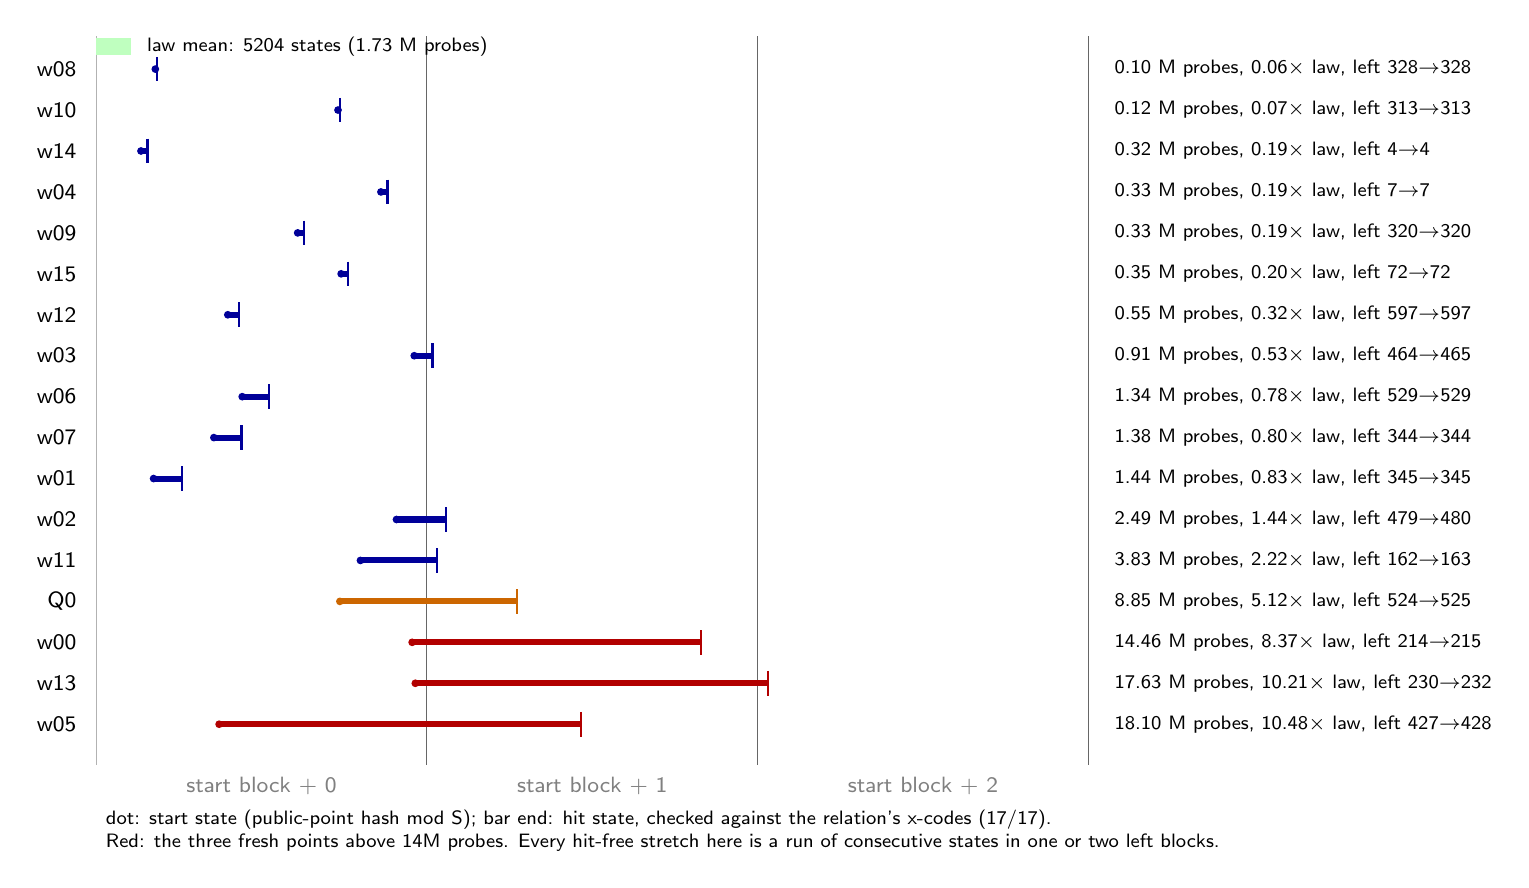
\begin{tikzpicture}[font=\sffamily\footnotesize,x=42mm,y=-5.2mm]
\draw[black!30] (0,-0.8) -- (0,17);
\node[gray] at (0.50,17.5) {start block + 0};
\draw[black!60] (1,-0.8) -- (1,17);
\node[gray] at (1.50,17.5) {start block + 1};
\draw[black!60] (2,-0.8) -- (2,17);
\node[gray] at (2.50,17.5) {start block + 2};
\draw[black!60] (3,-0.8) -- (3,17);
\fill[green!25] (0,-0.75) rectangle (0.1045,-0.35);
\node[anchor=west,font=\sffamily\scriptsize] at (0.1245,-0.55) {law mean: 5204 states (1.73 M probes)};
\node[anchor=east] at (-0.03,0) {w08};
\draw[line width=2.2pt,blue!60!black] (0.1789,0) -- (0.1848,0);
\fill[blue!60!black] (0.1789,0) circle (1.4pt);
\draw[blue!60!black,thick] (0.1848,-0.300000) -- (0.1848,0.300000);
\node[anchor=west,font=\sffamily\scriptsize] at (3.05,0) {0.10 M probes, 0.06$\times$ law, left 328$\to$328};
\node[anchor=east] at (-0.03,1) {w10};
\draw[line width=2.2pt,blue!60!black] (0.7312,1) -- (0.7384,1);
\fill[blue!60!black] (0.7312,1) circle (1.4pt);
\draw[blue!60!black,thick] (0.7384,0.700000) -- (0.7384,1.300000);
\node[anchor=west,font=\sffamily\scriptsize] at (3.05,1) {0.12 M probes, 0.07$\times$ law, left 313$\to$313};
\node[anchor=east] at (-0.03,2) {w14};
\draw[line width=2.2pt,blue!60!black] (0.1355,2) -- (0.1551,2);
\fill[blue!60!black] (0.1355,2) circle (1.4pt);
\draw[blue!60!black,thick] (0.1551,1.700000) -- (0.1551,2.300000);
\node[anchor=west,font=\sffamily\scriptsize] at (3.05,2) {0.32 M probes, 0.19$\times$ law, left 4$\to$4};
\node[anchor=east] at (-0.03,3) {w04};
\draw[line width=2.2pt,blue!60!black] (0.8610,3) -- (0.8807,3);
\fill[blue!60!black] (0.8610,3) circle (1.4pt);
\draw[blue!60!black,thick] (0.8807,2.700000) -- (0.8807,3.300000);
\node[anchor=west,font=\sffamily\scriptsize] at (3.05,3) {0.33 M probes, 0.19$\times$ law, left 7$\to$7};
\node[anchor=east] at (-0.03,4) {w09};
\draw[line width=2.2pt,blue!60!black] (0.6093,4) -- (0.6294,4);
\fill[blue!60!black] (0.6093,4) circle (1.4pt);
\draw[blue!60!black,thick] (0.6294,3.700000) -- (0.6294,4.300000);
\node[anchor=west,font=\sffamily\scriptsize] at (3.05,4) {0.33 M probes, 0.19$\times$ law, left 320$\to$320};
\node[anchor=east] at (-0.03,5) {w15};
\draw[line width=2.2pt,blue!60!black] (0.7407,5) -- (0.7621,5);
\fill[blue!60!black] (0.7407,5) circle (1.4pt);
\draw[blue!60!black,thick] (0.7621,4.700000) -- (0.7621,5.300000);
\node[anchor=west,font=\sffamily\scriptsize] at (3.05,5) {0.35 M probes, 0.20$\times$ law, left 72$\to$72};
\node[anchor=east] at (-0.03,6) {w12};
\draw[line width=2.2pt,blue!60!black] (0.3980,6) -- (0.4311,6);
\fill[blue!60!black] (0.3980,6) circle (1.4pt);
\draw[blue!60!black,thick] (0.4311,5.700000) -- (0.4311,6.300000);
\node[anchor=west,font=\sffamily\scriptsize] at (3.05,6) {0.55 M probes, 0.32$\times$ law, left 597$\to$597};
\node[anchor=east] at (-0.03,7) {w03};
\draw[line width=2.2pt,blue!60!black] (0.9618,7) -- (1.0169,7);
\fill[blue!60!black] (0.9618,7) circle (1.4pt);
\draw[blue!60!black,thick] (1.0169,6.700000) -- (1.0169,7.300000);
\node[anchor=west,font=\sffamily\scriptsize] at (3.05,7) {0.91 M probes, 0.53$\times$ law, left 464$\to$465};
\node[anchor=east] at (-0.03,8) {w06};
\draw[line width=2.2pt,blue!60!black] (0.4416,8) -- (0.5228,8);
\fill[blue!60!black] (0.4416,8) circle (1.4pt);
\draw[blue!60!black,thick] (0.5228,7.700000) -- (0.5228,8.300000);
\node[anchor=west,font=\sffamily\scriptsize] at (3.05,8) {1.34 M probes, 0.78$\times$ law, left 529$\to$529};
\node[anchor=east] at (-0.03,9) {w07};
\draw[line width=2.2pt,blue!60!black] (0.3559,9) -- (0.4391,9);
\fill[blue!60!black] (0.3559,9) circle (1.4pt);
\draw[blue!60!black,thick] (0.4391,8.700000) -- (0.4391,9.300000);
\node[anchor=west,font=\sffamily\scriptsize] at (3.05,9) {1.38 M probes, 0.80$\times$ law, left 344$\to$344};
\node[anchor=east] at (-0.03,10) {w01};
\draw[line width=2.2pt,blue!60!black] (0.1736,10) -- (0.2605,10);
\fill[blue!60!black] (0.1736,10) circle (1.4pt);
\draw[blue!60!black,thick] (0.2605,9.700000) -- (0.2605,10.300000);
\node[anchor=west,font=\sffamily\scriptsize] at (3.05,10) {1.44 M probes, 0.83$\times$ law, left 345$\to$345};
\node[anchor=east] at (-0.03,11) {w02};
\draw[line width=2.2pt,blue!60!black] (0.9080,11) -- (1.0586,11);
\fill[blue!60!black] (0.9080,11) circle (1.4pt);
\draw[blue!60!black,thick] (1.0586,10.700000) -- (1.0586,11.300000);
\node[anchor=west,font=\sffamily\scriptsize] at (3.05,11) {2.49 M probes, 1.44$\times$ law, left 479$\to$480};
\node[anchor=east] at (-0.03,12) {w11};
\draw[line width=2.2pt,blue!60!black] (0.7991,12) -- (1.0308,12);
\fill[blue!60!black] (0.7991,12) circle (1.4pt);
\draw[blue!60!black,thick] (1.0308,11.700000) -- (1.0308,12.300000);
\node[anchor=west,font=\sffamily\scriptsize] at (3.05,12) {3.83 M probes, 2.22$\times$ law, left 162$\to$163};
\node[anchor=east] at (-0.03,13) {Q0};
\draw[line width=2.2pt,orange!80!black] (0.7369,13) -- (1.2719,13);
\fill[orange!80!black] (0.7369,13) circle (1.4pt);
\draw[orange!80!black,thick] (1.2719,12.700000) -- (1.2719,13.300000);
\node[anchor=west,font=\sffamily\scriptsize] at (3.05,13) {8.85 M probes, 5.12$\times$ law, left 524$\to$525};
\node[anchor=east] at (-0.03,14) {w00};
\draw[line width=2.2pt,red!70!black] (0.9554,14) -- (1.8298,14);
\fill[red!70!black] (0.9554,14) circle (1.4pt);
\draw[red!70!black,thick] (1.8298,13.700000) -- (1.8298,14.300000);
\node[anchor=west,font=\sffamily\scriptsize] at (3.05,14) {14.46 M probes, 8.37$\times$ law, left 214$\to$215};
\node[anchor=east] at (-0.03,15) {w13};
\draw[line width=2.2pt,red!70!black] (0.9650,15) -- (2.0315,15);
\fill[red!70!black] (0.9650,15) circle (1.4pt);
\draw[red!70!black,thick] (2.0315,14.700000) -- (2.0315,15.300000);
\node[anchor=west,font=\sffamily\scriptsize] at (3.05,15) {17.63 M probes, 10.21$\times$ law, left 230$\to$232};
\node[anchor=east] at (-0.03,16) {w05};
\draw[line width=2.2pt,red!70!black] (0.3718,16) -- (1.4664,16);
\fill[red!70!black] (0.3718,16) circle (1.4pt);
\draw[red!70!black,thick] (1.4664,15.700000) -- (1.4664,16.300000);
\node[anchor=west,font=\sffamily\scriptsize] at (3.05,16) {18.10 M probes, 10.48$\times$ law, left 427$\to$428};
\node[anchor=west,font=\sffamily\scriptsize,align=left] at (0,18.6) {dot: start state (public-point hash mod S); bar end: hit state, checked against the relation's x-codes (17/17).\\ Red: the three fresh points above 14M probes. Every hit-free stretch here is a run of consecutive states in one or two left blocks.};
\end{tikzpicture}
\end{document}
